%%%%%%%%%%%%%%%%%%%%%%%%%
\section{\label{sec:rhs_nvt}Unbiased canonical ensemble ($NVT$) trials}
%%%%%%%%%%%%%%%%%%%%%%%%%

Canonical-ensemble trials are defined as trials that do not change the total number of particles of each type, $N_i$, the volume, $V$, or the temperature, $T$, and unbiased trials have transition probabilities that do not depend upon the configuration (e.g., not configurational bias).

In order to obtain trial acceptance in the $NVT$ ensemble, first the ratio of microstate probabilities (i.e., the first ratio in Eq.~\ref{eq:detailed_balance}), the probabilities of each microstate must be known proportionally with respect to the variables that change during the trial (e.g., only the coordinates, $\mathbf{r}$).
The probability of a microstate in the $NVT$ ensemble is proportional to \cite{allen_computer_1989, frenkel_understanding_2002}
\begin{equation}
\Pi \diff\mathbf{r}^N\diff\boldsymbol{\omega}^N \propto e^{-\beta U} \diff\mathbf{r}^N\diff\boldsymbol{\omega}^N,
\label{eq:rhs_nvt_pi}
\end{equation}
where $U$ is the total potential energy, $\beta=\frac{1}{k_B T}$, and $k_B$ is the Boltzmann constant.
The integration variables $\diff\mathbf{r}^{N}$ and $\diff\boldsymbol{\omega}^{N}$ are made explicit because these are the variables which change in an $NVT$ trial, and their randomly generated values for perturbations must be chosen uniformly (e.g., for $\diff\mathbf{r}$, choosing uniformly in each dimension, and for $\diff\boldsymbol{\omega}$, choosing uniformly on the surface of a unit sphere).
Because Eq.~\ref{eq:detailed_balance} requires information about only the ratio of microstate probabilities, we do not need to include any coordinate-independent terms that cancel when forming the ratio.
Thus, terms such as the partition function, the thermal de Broglie wavelength and the accounting of indistinguishability do not contribute to the $NVT$ ratio of probabilities.

Given Eq.~\ref{eq:rhs_nvt_pi}, the ratio of $NVT$ microstate probabilities, the first ratio in Eq.~\ref{eq:detailed_balance}, is given by
\begin{equation}
\frac{\Pi_n}{\Pi_o} = e^{-\beta\Delta U},
\label{eq:rhs_nvt}
\end{equation}
where $\Delta U = U_n - U_o$, $U_n$ and $U_o$ are the potential energies of the new and old state, respectively, and $N$, $V$ and $T$ are constant.
This expression is used for any trial that changes only the positions and orientations of the particles.

%%%%%%%%%%%%%%%%%%%%%%%%%
\subsection{\label{sec:lhs_translation}Particle translation trial}
%%%%%%%%%%%%%%%%%%%%%%%%%

An MC translation trial move is defined as follows.
A particle is randomly chosen among all of the mobile, non-fixed particles in the old microstate.
The total number of mobile particles is $N_m=\sum_i^{mobile} N_i$, where $i$ is the particle type.
The randomly chosen particle with position $\mathbf{r}_o$ in the old microstate is then translated by a random amount selected uniformly within $\pm\delta/2$ in each of $D$ dimensions, to a new position labeled $\mathbf{r}_n$, thereby defining the new microstate.

For this trial, the transition probability, $\alpha_{o\rightarrow n}$, may be obtained as the product of the transition probabilities for each step.
Each step that involves the generation of a random number should be considered.
In this translation trial, there are two such steps.
In the first, a particle is chosen randomly among $N_m$ mobile particles.
This means that the probability of choosing that particular particle, $1/N_m$, is the transition probability of the first step.
In the second step, $\mathbf{r}_n$ is chosen uniformly within a region of volume $\delta^D$.
Thus, the transition probability density of choosing $\mathbf{r}_n$ in the second step is $1/\delta^D$, and the transition probability is $\diff\mathbf{r}/\delta^D$.
In a computer experiment, positions may be determined only within machine precision, which is represented here by $\diff\mathbf{r}$.
%In theory, $\diff\mathbf{r}$ is included with the integral of the partition function.
Formally, $\diff\mathbf{r}$ is required to quantify the probability of choosing a position in continuous space.
Thus,
\begin{equation}
\alpha_{o\rightarrow n} = \frac{\diff\mathbf{r}}{N_m \delta^D}.
\label{eq:lhs_disp_forward}
\end{equation}

\begin{figure}
\begin{centering}
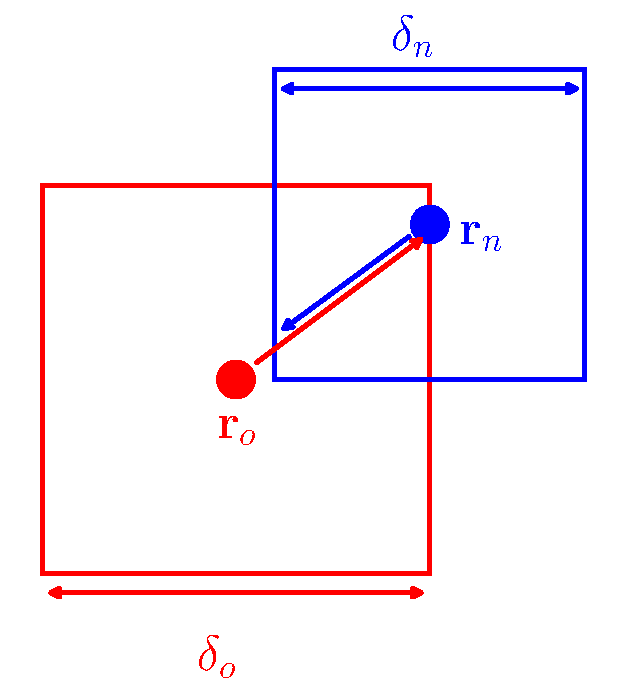
\includegraphics[width=6.5cm]{../figures/lhs_nvt.pdf}
\caption{
Detailed balance is violated if the tunable translation parameter, $\delta$, decreases.
If the particle is translated from the old position, $\mathbf{r}_o$, within $\delta_o$ in each dimension, then the particle may not be able to return to $\mathbf{r}_o$ in the reverse trial if the next translation is within $\delta_n<\delta_o$.
This is why $\delta$ should change only during equilibration and not during production simulations.
}
\label{fig:lhs_nvt}
\end{centering}
\end{figure}

In order to solve for the trial acceptance probability, $\chi$, the reverse trial transition probability from the new microstate to the old microstate, $\alpha_{n\rightarrow o}$, must also be obtained in order to utilize Eq.~\ref{eq:detailed_balance}.
The reverse transition must always be capable of returning to the old microstate; otherwise detailed balance is violated.
For example, detailed balance is violated if $\delta$ is tuned to reach a desired acceptance probability.
When $\delta$ is made smaller after a translation trial, it may be impossible for the next trial to reverse back to the old state, as illustrated in Fig.~\ref{fig:lhs_nvt}.
For this reason, $\delta$ should be changed only during equilibration and not during production simulations.

Throughout this article, we tabulate these forward and reverse transition probabilities, $\pi$, step-by-step with a corresponding table, as shown for a translation trial in Table~\ref{tab:lhs_translation}.
This table should indicate every use of a random number generator in both the forward and reverse transitions.
Again, the overall transition probability for a trial is the product of the probabilities for a given direction.

\begin{table}
\begin{center}
\begin{tabular}{|c|c|c|c|c|}
 \cline{1-2}\cline{4-5}
 \thead{Forward} & \thead{$\alpha_{o\rightarrow n}$} & & \thead{Reverse} & \thead{$\alpha_{n\rightarrow o}$}\\ [0.5ex]
 \cline{1-2}\cline{4-5}
 \makecell{Choose from $N_m$} & \makecell{$1/N_m$} & & \makecell{Choose from $N_m$} & \makecell{$1/N_m$} \\
 \cline{1-2}\cline{4-5}
 \makecell{Choose $\mathbf{r}_n$} & \makecell{$\diff\mathbf{r}/\delta^D$} & & \makecell{Choose $\mathbf{r}_o$} & \makecell{$\diff\mathbf{r}/\delta^D$} \\
 \cline{1-2}\cline{4-5}
\end{tabular}
\caption{Translation transition probabilities.}
\label{tab:lhs_translation}
\end{center}
\end{table}

The reverse transition probability is given by
\begin{equation}
\alpha_{n\rightarrow o} = \frac{\diff\mathbf{r}}{N_m \delta^D}.
\label{eq:lhs_disp_rev}
\end{equation}
Substituting Eqs.~\ref{eq:rhs_nvt}, \ref{eq:lhs_disp_forward} and \ref{eq:lhs_disp_rev} into Eq.~\ref{eq:detailed_balance} yields,
\begin{equation}
\chi = e^{-\beta\Delta U}
\label{eq:lhs_translate}
\end{equation}
for the Metropolis acceptance of translation trials.

\begin{figure}
\lstinputlisting[
language=Python,
label={sim:nvt_harmonic},
caption={MC simulation of a single particle in one dimension attached to a harmonic spring using Python 3, where the statistics module is provided in Section~\ref{sec:block_av}. Note that a random number generator seed of "43279857" is provided so that the simulation is reproducible.}
]{../codes/nvt_harmonic.py}
\end{figure}

Code Block~\ref{sim:nvt_harmonic} tests Eq.~\ref{eq:lhs_translate} for a single particle subject to an external harmonic potential centered about the origin in one dimension.
The expected average position is the origin.
Also, according to the equipartition theorem, the expected average energy is $0.5k_BT$.

One major difference between MD and MC is that all particles are moved simultaneously in one MD time step, while typically only a single particle is moved in one MC trial.
If multiple particles were moved in one MC trial, then only one unfavorable overlap from one particle could cause the rejection of an entire trial.
Thus, it is typically more efficient to perturb only one particle at a time.
However, there are special cases where it is still efficient for more than one particle to move in a single trial, as discussed in Section~\ref{sec:lhs_cluster}.

The tunable translation parameter may have an optimal value in a dense fluid.
Larger translations are likely to overlap with another particle, while smaller translations are more correlated with the old microstate, reducing sampling efficiency.
Tunable translation parameters are optimized by changing $\delta$ during an equilibration period to achieve a desired acceptance, often $25$ $\%$ \cite{kolafa_optimization_1987, jacucci_comparing_1984, chapman_metropolis_1985, mountain_quantative_1994, hatch_parallel_2020}.
Although Metropolis \textit{et. al} \cite{metropolis_equation_1953} used 50 \%, it seems that higher efficiencies may be achieved with slightly lower acceptances for particle translation because rejects can be less expensive (e.g., hard overlap detected, updating neighbor lists, etc.) and larger translations can lead to large configuration changes, although too low of acceptance also runs the risk of poor sampling.

An efficient implementation may have a translation parameter, $\delta_i$, specifically tuned for each particle type, $i$.
This could be important to improve sampling in cases where the particle sizes or interactions are different.
In addition, particles are chosen from all mobile particles, $N_m$.
An alternative would be to define separate trials that select among specific particle types.
In that case, if there are more particles of one type than another, the species with fewer numbers could have a relatively larger probability of translation.
The relative efficiency of this alternative approach compared to the one derived here is beyond the scope of this article.
If the minor species is of more interest, the alternative could be more efficient.
On the other hand, inefficiencies could arise if the minor species were caged in solvent that was not as well sampled.
%Although these trials could be assigned different weights to correct this relative probability, such weights would need to be recomputed when the number of particles changes.

The goal of translation trials is to give every particle a chance to move.
In principle, any state may be visited, which is a key element of the ergodic hypothesis.
Although sequential updates have been shown to converge faster than random updates in an Ising model, sequential updates break detailed balance and follow a weaker balance condition \cite{ren_acceleration_2006}.
Trials that do not obey detailed balance are outside the scope of this article.

This translation algorithm could also be carefully modified to select particles only in a specific region of space.
But detailed balance violations could occur if the set of available particles changes.
For example, it is possible for the translation to take a particle out of this region.
If so, the trial must be immediately rejected, because the particle that was taken out of the region cannot be chosen for the reverse transition and therefore detailed balance is violated.

%%%%%%%%%%%%%%%%%%%%%%%%%
\subsection{\label{sec:lhs_rotation}Particle orientation-change trial}
%%%%%%%%%%%%%%%%%%%%%%%%%

Orientations are typically fixed during particle translation trials so as not to introduce a second tunable parameter for orientation moves that cannot be decoupled from the translation parameter during optimization.
Instead, the orientation of a single particle may be perturbed in a separate trial move.
A robust and intuitive way to accomplish this is via the axis-angle method: (1) a particle is randomly chosen among $N_m$ mobile particles; (2) a rotation axis $\hat {\bf u}$ is generated by sampling uniformly on the surface of a sphere (Sec.~\ref{sec:unit_sphere}); (3) a rotation angle $\theta$ is generated uniformly on $\pm\delta\theta_{max}/2$ (with $\delta\theta_{max}$ a tunable parameter).
With the rotation so defined, a rotation matrix can be computed
\begin{equation}
\mathbf{R} =
\begin{bmatrix}
C + (1 - C) u_x^2 & (1 - C) u_x u_y - S u_z & (1 - C) u_x u_z + S u_y \\
(1 - C) u_y u_x + S u_z & C + (1 - C) u_y^2 & (1 - C) u_y u_z - S u_x \\
(1 - C) u_z u_x - S u_y & (1 - C) u_z u_y + S u_x & C + (1 - C) u_z^2
\end{bmatrix}
\label{eq:rotation_matrix}
\end{equation}
where $C =\cos\theta$ and $S = \sin\theta$.
The new coordinate of interaction site $j$ on particle $i$ at ${\bf r}_i$ is given by ${{\bf r}_{ij,{\rm n}}={\bf r}_{i}}+{\mathbf R}({\bf r}_{ij,{\rm o}}-{\bf r}_i)$.
If the particle's centroid is chosen for ${\bf r}_i$, then the centroid will be unchanged by the rotation (complementing the translation move, which leaves the orientation unchanged).
However, using the centroid for ${\bf r}_i$ is not a requirement; any well-defined center for the rotation may be employed (e.g., the position of a specific interaction site).

Alternatively, if the orientation coordinate is held explicitly (e.g., as a quaternion), then it can be updated from $\hat{\bf u}$ and $\theta$ using an appropriate formula.

%Axis-angle is suitable for orientation displacement of particles of any symmetry. However, it is not suitable for generating a random orientation from scratch, i.e. by selecting $\delta = 2\pi$. Generating a random quaternion is best for this.
Regardless of the selected center for the rotation, the transition probabilities are given in terms of the axis-angle selection process outlined above.
The elements of the transition probabilities for the particle orientation trial are summarized in Table~\ref{tab:lhs_rotation}.
Together they yield the forward and reverse probabilities, which in this case are again equal
\begin{equation}
  \alpha_{o\rightarrow n}=\alpha_{n\rightarrow o} = \frac{\diff\mathbf{\omega}\diff\theta}{N_m 4\pi\delta\theta_{max}}.
\label{eq:lhs_rhs_rot_fwdrev}
\end{equation}

\begin{table}
\begin{center}
\begin{tabular}{|c|c|}
 \hline
 \thead{Forward} & \thead{$\alpha_{o\rightarrow n}$} \\ [0.5ex]
 \hline
 \makecell{Choose from $N_m$} & \makecell{$1/N_m$} \\
 \hline
 \makecell{Choose rotation axis} & \makecell{$\diff\boldsymbol{\omega}/4\pi$} \\
 \hline
  \makecell{Choose rotation angle} & \makecell{$\diff\theta/\delta\theta_{max}$} \\
 \hline\hline
 \thead{Reverse} & \thead{$\alpha_{n\rightarrow o}$}\\ [0.5ex]
 \hline
 \makecell{Choose from $N_m$} & \makecell{$1/N_m$} \\
 \hline
 \makecell{Choose rotation axis} & \makecell{$\diff\boldsymbol{\omega}/4\pi$} \\
 \hline
  \makecell{Choose rotation angle} & \makecell{$\diff\theta/\delta\theta_{max}$} \\
 \hline
\end{tabular}
\caption{Orientation-change transition probabilities.}
\label{tab:lhs_rotation}
\end{center}
\end{table}

Substituting Eq.~\ref{eq:rhs_nvt} into Eq.~\ref{eq:detailed_balance} and using the transition probabilities in Table~\ref{tab:lhs_rotation} yields,
\begin{equation}
\chi = e^{-\beta\Delta U}
\label{eq:lhs_rotate}
\end{equation}
for the Metropolis acceptance of particle orientation changes.
To simplify notation, all remaining trial moves which include changes in orientation will simply refer to these transition probabilities as $P_{\omega n}$ and $P_{\omega o}$ for the new and old states, respectively.

A larger tunable parameter, $\delta\theta_{max}$, leads to a larger rotation, and thus $\delta\theta_{max}$ may be tuned in the same manner as the translation tunable parameter to reach a target acceptance for each species.
To avoid violating detailed balance, this tunable parameter should remain constant during the production simulations for the same reason as shown in Fig.~\ref{fig:lhs_nvt}.

If desired, generation of orientations from scratch, without perturbing on an existing orientation, is best accomplished by random generation of a quaternion.
An example of randomly picking quaternions, and thus orientations, is shown in Section~\ref{sec:unit_sphere}.

Code Block~\ref{sim:orientation_trials} tests Eqs.~\ref{eq:rotation_matrix} and \ref{eq:lhs_rotate} with the simulation of the orientation of a single rigid body given by two orthogonal unit vectors in $3$ dimensions.
Because there is no energy of interaction, the unit vectors are expected to be uniformly distributed on the surface of a sphere.
In spherical coordinates, this manifests as a uniform distribution of the azimuthal angle $\in [-\pi,\pi]$, which is defined as the angle between the x-axis and the projection of the vector on the x-y plane, and a sine distribution for the polar angle $\in [0,\pi]$, which is the angle between the z-axis and the vector.
While this azimuthal and polar angle of the first vector fully specifies the orientations of rigid bodies with an axis of symmetry, generic rigid bodies also require analysis of a third angle.
That third angle was chosen to be the azimuthal angle of the second vector in the reference frame of the first vector.
The reference frame was defined by the minimal rotation of the coordinate axes such that the z-axis aligns with the first vector.
These analytical expectations are compared against the MC simulation in Fig.~\ref{fig:orientation_trials}.

\begin{figure}
\lstinputlisting[
language=Python,
label={sim:orientation_trials},
caption={MC simulation of a single rigid body represented by two orthogonal unit vectors in three dimensions implemented in Python 3 using $5\times 10^5$ random angular displacements with $\delta\theta_{max}=\pi/10$. Angle distributions were computed over $300$ equally-spaced bins with $20$ independent simulations (totaling $10^7$ MC trials) to compare against theoretical expectations with approximately 68 \% of the distribution within one standard deviation.}
]{../codes/orientation_trials.py}
\end{figure}

\begin{figure}
\begin{centering}
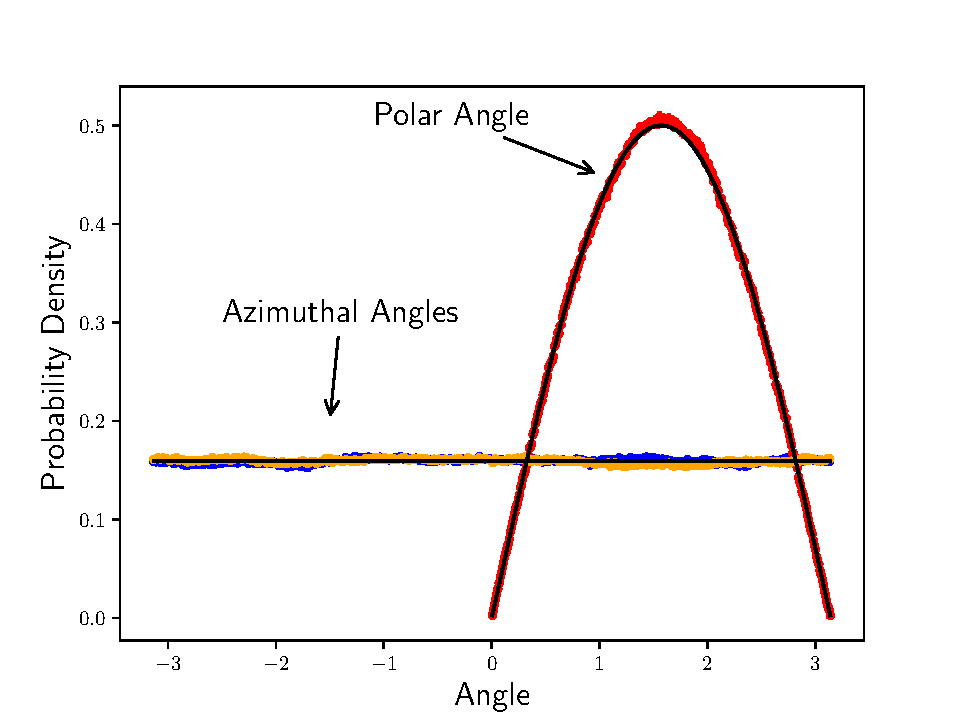
\includegraphics[width=8.5cm]{../figures/orientation_trials.pdf}
\caption{
  The (blue) azimuthal and (red) polar probability distributions of the first vector and (orange) azimuthal angle of the second vector in the reference frame of the first vector from MC simulations described in Code Block~\ref{sim:orientation_trials} with error bars from the standard deviation of the mean of $20$ independent simulations, and analytical expectations shown by the black lines.
\label{fig:orientation_trials}
}
\end{centering}
\end{figure}
%If desired, generation of orientations from scratch, without perturbing on an existing orientation, is accomplished by random generation of a quaternion \cite{vesely_angular_1982}.
%An example of randomly picking quaternions, and thus orientations, is shown in Section~\ref{sec:unit_sphere}.

%As a simple example, consider choosing a second site of a dimer that is bonded to the first with $k$ randomly generated positions according to the Boltzmann weighted potential, $U_{bond}$.
%In this case,
%\begin{equation}
%P_{\omega n}=\frac{e^{-\beta U_{bond}}}{W_n}
%\label{eq:pomegan}
%\end{equation}
%\begin{equation}
%W_n = \sum_k e^{-\beta U_{bond,k}}.
%\end{equation}
%Substituting Eq.~\ref{eq:pomegan} into \ref{eq:lhs_rotate}
%where the numerator removes the bonded energy from the total energy in Eq.~\ref{eq:lhs_rotate} so that only intermolecular energies are considered in the final acceptance, and the denominator is the usual Rosenbluth factor.
